\chapter{Experiments and Results}
Description generall
limiations of work

\section{Experiments on the Moons-Circles Dataset}
The first round of experiments is dedicated to finding out what conditions are required, such that the network separates.
During a preliminary exploration phase, some scenarios where the network indeed separates were found.
Yet, they were sparse and could not be easily interpreted.
Therefore, in this step, the knowledge gained from the initial experiments is put to use.
A systematic evaluation of the relationship between network size and splitting behavior was conducted.

To enable comparison between networks of different sizes, the network extension technique described in REF was used.
First, an extensive experiment with a network architecture of $(4,8,8,2)$ was conducted.
To expand the range of the results, two additional experiments were executed, which were slightly smaller to lower computational cost.
One experiment is done on a network with only one hidden layer, concretely with a shape $(4,20,2)$, and the other experiment on a network with three hidden layers, a shape of $(4,4,4,4,2)$.
All hyperparameters are shared amongst the three experiments.
The only difference is the pruning target, which is derived from the network architecture.

For all three experiments, the pruning rate was set to $0.32$.
The chosen value, while somewhat arbitrary, was selected by promising results on preliminary tests.
\textcite{LTH} used a pruning rate of $0.2$ in the original experiments for the fully connected feed-forward network trained on the MNIST dataset.
However, with a larger pruning rate, a larger space of network sizes can be covered with the same number of iterations, which is why the larger pruning rate of $0.32$ was selected.

\begin{table}[ht]
    {
    \sffamily
    \caption{
    In this table, the parameter trajectories and the corresponding hidden dimension of the network are displayed for each extension level. 
    Parameter trajectory is in each respective `param' column and the number of hidden neurons per hidden layer in the column `hidden dim'.
    At the extension level zero, the base model values are displayed.
    }\label{tab:trajectory}
    \begin{tabular}{rrrrrrr}
    \toprule
    Lvl & shape (1) & param (1) & shape (2) & param (2) & shape (3) & param (3) \\
    \midrule
    0 & 20 & 120 & 8 & 112 & 6 & 108 \\
    1 & 29 & 174 & 10 & 160 & 8 & 176 \\
    2 & 43 & 258 & 13 & 247 & 10 & 260 \\
    3 & 64 & 384 & 16 & 352 & 12 & 360 \\
    4 & 94 & 564 & 20 & 520 & 15 & 540 \\
    5 & 138 & 828 & 25 & 775 & 19 & 836 \\
    6 & 202 & 1212 & 31 & 1147 & 23 & 1196 \\
    7 & 297 & 1782 & 38 & 1672 & 29 & 1856 \\
    8 & 437 & 2622 & 47 & 2491 & 35 & 2660 \\
    9 & 643 & 3858 & 57 & 3591 & 43 & 3956 \\
    10 & 946 & 5676 & 70 & 5320 & 52 & 5720 \\
    11 & 1391 & 8346 & 85 & 7735 & 63 & 8316 \\
    12 & 2046 & 12276 & 104 & 11440 & 77 & 12320 \\
    13 & 3009 & 18054 & 127 & 16891 & 94 & 18236 \\
    14 & 4425 & 26550 & 154 & 24640 & 114 & 26676 \\
    15 & 6507 & 39042 & 188 & 36472 & 139 & 39476 \\
    16 & 9569 & 57414 & 229 & 53815 & 169 & 58136 \\
    17 &   &   & 278 & 78952 &   &   \\
    18 &   &   & 337 & 115591 &   &   \\
    19 &   &   & 410 & 170560 &   &   \\
    20 &   &   & 498 & 250992 &   &   \\
    21 &   &   & 604 & 368440 &   &   \\
    22 &   &   & 733 & 541687 &   &   \\
    23 &   &   & 890 & 797440 &   &   \\
    24 &   &   & 1080 & 1172880 &   &   \\
    25 &   &   & 1310 & 1723960 &   &   \\
    \bottomrule
    \end{tabular}
    }
\end{table}

\subsection{Two hidden layers}\label{two-hidden}
The first experiment was an extensive exploration of different model sizes by extending the network.
The base network, which is the network that is used as a base for extending, has the shape $(4,8,8,2)$.
This architecture has 112 weights, which is also used as the pruning target.
The network architecture indicated by the number of neurons per hidden layer and the respective number of weights are displayed in table~\ref{tab:trajectory}.
The network is extended up to 25 times.
At the extension level 25, the network has a shape of $(4,1310,1310,2)$, with 1.723.960 weights.
The number of extension levels corresponds to the number of pruning levels the network goes through.

Overall pruning levels, the network might separate into two networks or lose one of the inputs or outputs, which is called `degrading'.
For the experiments described here, the run is stopped as soon as the network degrades to avoid unnecessary computational effort.
After each pruning level, the network is evaluated to check if it is separated or degraded.
When looking at this throughout all pruning levels, there are four different scenarios for a network:

\begin{enumerate}
    \item separated (and not degraded)\\
    The network separates at some pruning level. 
    It does not degrade at any later level. 
    \item separated and later degraded \\
    The network splits at some point and has all input and output nodes.
    At a later level, the network degrades (it loses at least one input or output).
    \item degraded (and not separate before) \\
    The network degrades before it can separate.
    \item interconnected-not separated and not degraded \\
    The network does neither separate nor degrade. 
    The result is a single network that contains all input and output nodes of all tasks.
\end{enumerate}

\begin{figure}[ht]
    \centering
    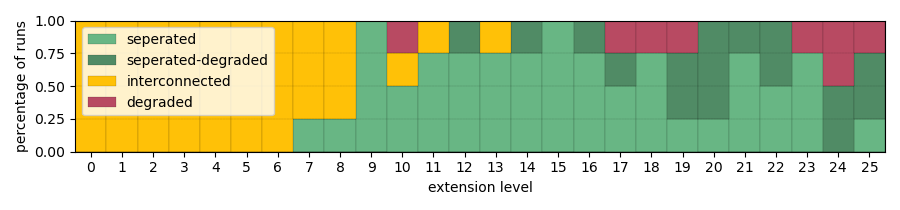
\includegraphics[width=1.0\linewidth]{2-layer-histogram-split-behaviour.png}
    \caption{
        This figure depicts the proportional stacked area chart for the network with two hidden layers.
        On the x-axis, the extension level is displayed. 
        Along the y-axis, the percentage of runs per category is shown.
        Each color determines the category that the run belongs to.
        }\label{fig:2laxer-histogram}
\end{figure}

At each extension level, the runs are repeated with four different seeds for the network initialization.
The results are displayed in figure~\ref{fig:2laxer-histogram}.
The figure is a proportional stacked area chart.
Each scenario described above is encoded with a color.
On the x-axis, the extension levels are shown.
On the y-axis, the percentage of networks in each category can be viewed.
A clear pattern in the data is, that the network separates for the first time with at least 7 pruning levels.
The shape and number of weights at that level are $(4,38,38,2)$ and 1672 respectively, which is $~15$ times the number of weights compared to the base model. 
Starting at shape $(4,57,57,2)$ or extension level 9, which represents an increase of $~32$-times, the majority of the networks separate.
Up until the 6th extension level, no network separates or degrades. 
However, if the network were pruned further, at some point every network would degrade.
Therefore it is also reasonable to assume that some of the networks that are still interconnected after all pruning iterations would separate well if they were pruned to less weights.

Another interesting observation is that only after extension level 10, do the networks begin to degrade.
What follows from the data is the more extension levels, the more likely it is that a network degrades, either before or after it separates.

One possible explanation for this is that at each pruning level, a certain number of `inactive weights' are produced.
As noted in \autocite{HanEtAl15, AllAlivePruning}, this is a known phenomenon.
However, since no regularisation is used in these experiments, the inactive weights do not decrease in magnitude.
Rather, they are frozen with their last value.
If more inactive parameters are created at each pruning level than pruned, the percentage of inactive weights in the network grows over the iterations.
Therefore, the more pruning levels the network experienced, the less of its available, unpruned parameters are active.
This effectively makes the network smaller, which in turn makes it more likely to separate or degrade.

\begin{figure}[ht]
    \centering
    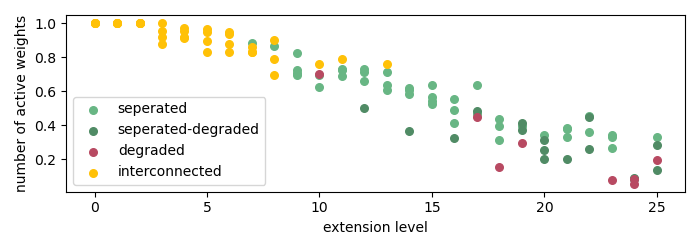
\includegraphics[width=1.0\linewidth]{2-layer-compund-damage.png}
    \caption{
        The figure depicts the number of active weights after the last pruning iteration of extended networks.
        On the x-axis, the extension level is displayed.
        On the y-axis, the number of active weights at that level.
        A clear pattern emerges, showing a correlation between the number of pruning iterations and the number of active weights in the final network.
    }\label{fig:collateral_damage}
\end{figure}

This effect is visible in figure~\ref{fig:collateral_damage}.
The colors are encoded in the same way as in figure~\ref{fig:2laxer-histogram}.
Each dot is a single run. 
The x-axis represents the extension level.
On the y-axis, the number of active weights after the last pruning level is displayed.
Important to note is that when a network degrades (red), the run is immediately stopped.
Therefore in this graph, the degraded networks might have larger numbers of active weights, compared to other networks that were pruned for the total amount of levels.
However, even with this caveat, a clear trend is visible.
The more pruning levels the network experiences, the smaller the percentage of the active network weights.
For some networks that were extended to 20 or more levels, the final percentage of active weights in the network is only $\sim20$ percent, which translates to only $\sim22$ active weights.

Techniques like L1-Regularisation used in \autocite{HanEtAl15} or All-Alive-Pruning \autocite{AllAlivePruning} could counteract this effect of compounding inactive parameters.
However, this is a topic for future research and is not addressed in this thesis. 

\subsection{When do networks separate?}
One question regarding the separation of a network is, at what level it separates.
What is the number of available weights the network has at the level when it splits?
How does the number of extension levels / the network size influence the iteration when it splits?

\begin{figure}[ht]
    \centering
    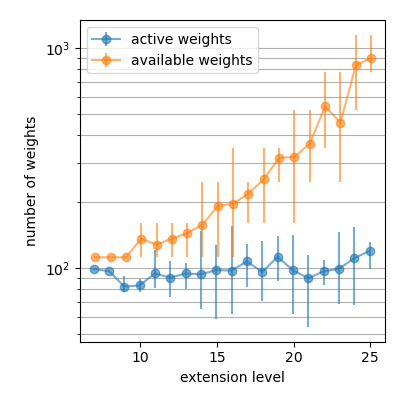
\includegraphics[width=.5\linewidth]{2-layer-active-available-at-split-log.png}
    \caption{
        The figure depicts the number of available weights / prunable weights (orange) and the number of active weights (blue) at the iteration when the networks first split.
        Each dot represents an average over four runs with different seeds.
        The error bars indicate the maximum and minimum value of the different runs.
        While the number of available weights at the split iteration increases, the number of active weights stays fairly constant.
        Logarithmic.
    }\label{fig:2l-active-split}
\end{figure}

Interestingly, when extending the network more, it tends to split into earlier pruning levels.
In figure~\ref{fig:2l-active-split}, the number of available/unpruned weights (orange) weights at each pruning level is displayed.
Only the range of extension levels where the network is separated is displayed.
Each point on the line represents an average of three runs, repeated with different seeds for the network initialization.
The error bars depict the minimum and maximum values among those three repeated runs.
The graph is shown on a logarithmic scale, and the increase follows almost an exponential curve.
The earlier the network separates in terms of pruning levels, the more unpruned weights it has.
However, when looking at the number of active weights the networks have at the iteration they split, the curve does not have the same exponential growth trajectory.
It increases slightly but almost remains flat, covering a narrow range of around 80 to 120 weights.

TODO: revise. Does this make any sense?
This data indicates that the number of active weights is an important quantity to splitting.
Since the active subgraph is indeed the graph on which the splitting is checked, this seems plausible.
A certain `barrier' might be inherent to each combination of network architecture, dataset, and hyperparameters.
Given a dataset where there is exactly zero correlation between the two tasks might move the barrier towards a larger number of edges where the network is likely to split.
A slight correlation, which is probably also the case in the Moons-Circles dataset, might move the barrier lower.
Some hyperparameters or optimizers also might move the barrier, by being better suited to remove weights that connect the tasks.
For instance, techniques like L1 regularisation might move the barrier up, due to more efficient removal of weights that do not increase in magnitude, but also do not decrease on their own.
These are all questions for further research to tackle.
 
\subsection{What makes the networks separate?}
As seen in figure~\ref{fig:2laxer-histogram}, the network starts to split at 7 extension levels and a network shape of $(4,38,38,2)$, with 1672 weights.
However, it is not obvious what the main contributor to network splitting is.
To gain a better understanding of that phenomenon an experiment was conducted that compares different combinations of pruning levels, network size, and pruning rate.
For this experiment, four architectures were selected.
One network with shape $(4,31,31,2)$ (extension level 6), which did not separate in any run.
A network with 38 and 48 hidden neurons (extension levels 7 and 8), where only one in four networks is separated.
And finally a network with 57 hidden neurons, where all four runs have separated.
This range of architectures is assumed to encompass a critical area, due to the change in splitting behavior.
Further, each of the four architectures was trained with 0 to 10 pruning levels.
The pruning target is fixed at 112, such that all networks end up at the same number of prunable parameters after the last pruning level.
Therefore, the pruning rate is variable depending on network size and number of levels.
Each combination of network size and number of pruning levels was repeated four times, with different seeds for the network initialization.

\begin{figure}[ht]
    \centering
    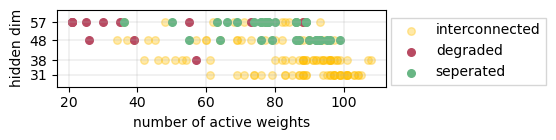
\includegraphics[width=1.0\linewidth]{grid-2-layer-eval-abs.png}
    \caption{This Figure depicts the network size by the number of neurons per hidden layer (hidden dim) against the number of active weights after all pruning levels.
    The colors denote if the network separated, degraded or stayed connected.}\label{fig:grid-1}
\end{figure}

In figure~\ref{fig:grid-1} the impact of network size is demonstrated.
On the y-axis, the size of the network is encoded by its hidden dimension.
On the x-axis, the number of active weights after all pruning levels is depicted.
Each dot represents one run of the experiment.
Regarding the two smaller networks with hidden dimensions 31 and 38, none of the networks separated. 
Increasing the number of pruning levels and decreasing the pruning rate did not result in a separated network.
On the other hand, the two larger networks indeed split.

These results indicate, that there is a phase change in the ability of the network to separate and that it has to have a certain minimum of overparameterization.
There is no hard boundary, but probably a significant increase in the likelihood of splitting when the network exceeds a certain size.

\begin{figure}[ht]
    \centering
    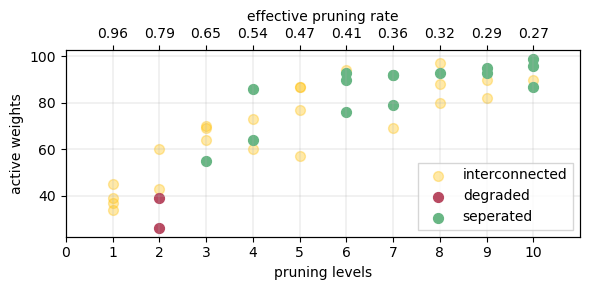
\includegraphics[width=1.0\linewidth]{grid-2-layer-pruning-rate-48-hd.png}
    \caption{This Figure depicts the network with shape $(4,48,48,2)$.
    The network was trained with different numbers of pruning levels, which is displayed along the bottom x-axis.
    On the top x-axis the associated pruning rate is displayed.
    The y-axis shows the number of active weights after all pruning levels.
    }\label{fig:grid-2}
\end{figure}

To investigate the influence of pruning levels and pruning rate, the splitting behavior of the network with hidden dimension 48 is depicted in figure~\ref{fig:grid-2}.
Since the pruning target and the network size are fixed, the pruning rate has to change when increasing the number of pruning levels.
On the bottom x-axis, the number of pruning levels is depicted, and on the top x-axis, is the corresponding pruning rate.
On the y-axis, the number of active weights after all pruning levels is depicted.
With more pruning levels and a lower pruning rate, the network is more likely to separate.
Also, a seemingly contradicting trend to figure~\ref{fig:collateral_damage} is visible, namely that the number of active weights increases with more pruning levels.
The difference to the previous experiment is, that while the number of pruning levels increases in both cases, the pruning rate decreases in in this experiment, visible in figure~\ref{fig:grid-2}. In the experiment depicted in figure~\ref{fig:collateral_damage}, the pruning rate is constant, while the network size increases.

However, this data also indicates that there is a certain phase change in the likelihood of splitting.
Since the pruning rate and the number of pruning levels are two tightly interlinked parameters, it is hard to examine them in isolation.
The largest pruning rate where a network separated was $\sim0.65$. 
With pruning rates lower than $\sim0.41$, the networks consistently separate.
The data indicates that more pruning levels with lower pruning rates are generally favorable to network splitting.
\textcite{LTH} already note that iterative pruning leads to smaller lottery tickets than one-shot pruning.
It is reasonable to assume, that the same phenomenon takes place with regards to network splitting.
Less pruning levels versus lower pruning rates represent a trade-off between favorable conditions and computational cost.

\subsection{One and Three hidden layers}
To gain a wider picture of the effects studied concerning the network with two hidden layers, the same experiments were conducted on networks with one and three hidden layers.
As shown in table~\ref{tab:trajectory}, the networks were only extended for 15 and 17 levels instead of 25. 
This is due to computational constraints. As the networks get larger and the number of pruning levels is higher, the computational effort increases significantly.

For the network with one hidden layer a base with shape $(4,20,2)$ was selected.
It has a similar number of weights compared to the base network with two layers.

\begin{figure}[ht]
    \centering
    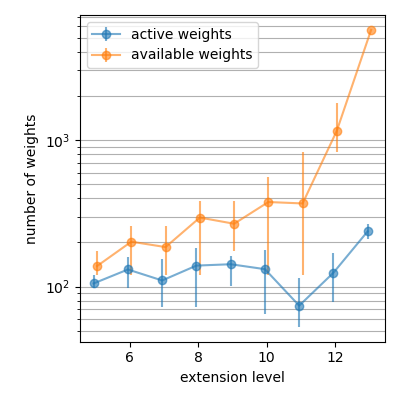
\includegraphics[width=0.5\linewidth]{1-layer-active-available-at-split-log.png}
    \caption{This Figure depicts the network with shape $(4,20,2)$.
    On the x-axis, the number of levels the network was extended to is displayed, which is also the number of pruning levels.
    The orange line shows the number of unpruned weights that are available to the network at each iteration.
    The blue line indicates the number of active weights.
    The error bars show the minimum and maximum values from the different experiments.
    }\label{fig:1layer-active}
\end{figure}

\begin{figure}[ht]
    \centering
    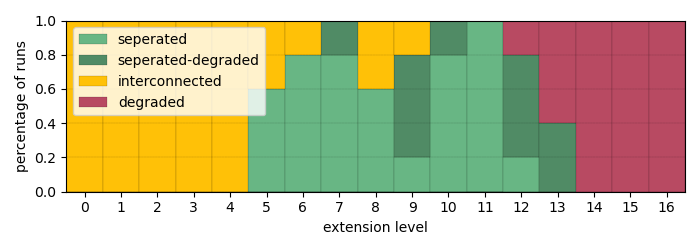
\includegraphics[width=1.0\linewidth]{1-layer-histogram-split-behaviour.png}
    \caption{
        This figure depicts the proportional stacked area chart for the network with one hidden layer.
        On the x-axis, the extension level is displayed. 
        Along the y-axis, the percentage of runs per category is shown.
        Each color determines the category that the run belongs to.
    }\label{fig:1layer-histogram}
\end{figure}

In figure~\ref{fig:1layer-histogram}, the same plot as for the two-layer experiment is presented.
A similar trend is visible.
After a certain number of pruning levels and network size, the networks begin to consistently split.
Given a few more pruning levels, the networks start to degrade more often, either before or after they separate.
Interestingly, at iteration 12, the network starts to degrade more often before it splits.
Beginning at 14 extension levels, where the networks are the largest, they never split and only degrade.
The reason for this behavior is unknown.
It might be that the networks with more layers also exhibit such behavior at even higher extension levels. 

In figure~\ref{fig:1layer-active}, the number of active weights (blue) in the network versus the number of available, unpruned weights (orange) is compared.
Only the range of extension levels where the network is separated is displayed.
The graph is displayed on a logarithmic scale.
Similarly to the experiment with two layers, the networks split in earlier iterations when they are larger and have more pruning levels.
This is indicated by the larger number of available weights, which directly correlate with the pruning level.
The number of active weights remains in a fairly tight range between 70 and 120 active weights.

Regarding the network with three hidden layers, the results are similar.
\begin{figure}[ht]
    \centering
    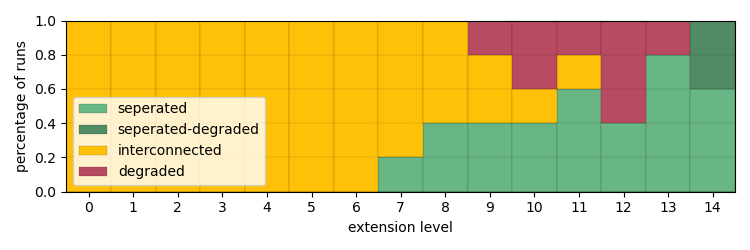
\includegraphics[width=1.0\linewidth]{3-layer-histogram-split-behaviour.png}
    \caption{
        This figure depicts the proportional stacked area chart for the network with three hidden layers.
        On the x-axis, the extension level is displayed. 
        Along the y-axis, the percentage of runs per category is shown.
        Each color determines the category that the run belongs to.
    }\label{fig:3layer-histogram}
\end{figure}

\begin{figure}[ht] 
    \centering
    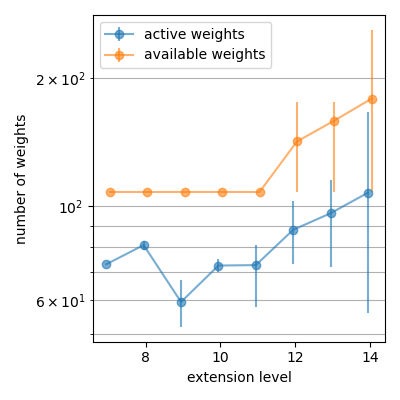
\includegraphics[width=0.5\linewidth]{3-layer-active-available-at-split-log.png}
    \caption{
        The figure depicts the number of available weights / prunable weights (orange) and the number of active weights (blue) at the iteration when the networks first degrades.
    Each dot represents an average over five runs with different seeds.
    The error bars indicate the maximum and minimum value of the different runs.
    }\label{fig:3layer-active}
\end{figure}

In figure~\ref{fig:3layer-histogram} the splitting behaviour is depicted.
A similar effect occurs but unlike the single-layer network, the network does not stop to separate in the range that was tested. 

In figure~\ref{fig:3layer-active} the number of active weights and the number of available weights is displayed.
Only the range of extension levels where the network is separated is displayed.
The networks at extension level 7 until 11 all split at the last pruning level, which can be deducted by the number of available parameters which is equal to the pruning target of 108.
The number of active weights is slightly lower than in the other experiments.
Generally, the same pattern can be seen, with a slightly more pronounced increase in active weights for larger networks.

\subsection{How do networks separate?}
Another open question is, what the process of separation looks like.
In the beginning, it is not yet clear which weight and neuron belongs to which task.
One available option, however, is to view the network from the perspectives of the inputs and outputs.
The input and output features are the only parts of the network that can already be ascribed to a task when it is fully connected.
This enables us to determine the degree to which the neighboring layers have separated as well.

For instance, regarding the simple Moons-Circles dataset, there are two output neurons.
Each neuron in the penultimate layer has two outgoing connections: one to the Circles-output and one to the Moons-output.
When one of the connections is pruned, the neuron and all its incoming connections are automatically part of the task the unpruned weight is connected to.

The number of neurons that are only connected to one of the outputs of one task is denoted $N_{decided}$.
The number of neurons that are connected to more than all tasks is denoted $N_{undecided}$.
The degree of separation is determined by 
\[
\frac{N_{decided}}{N_{decided}+N_{undecided}}
\]

This calculation can be done from either the side of the inputs or the outputs and it works in the same way.
Only if a layer has at least one neuron that has `decided' to which task it belongs, neurons in the next layer can `decide' as well.

\begin{figure}[ht]
    \centering
    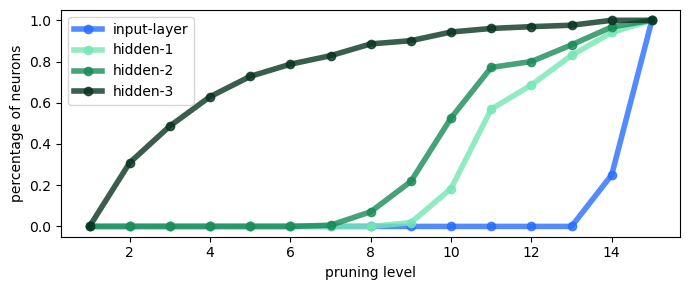
\includegraphics[width=0.9\linewidth]{output-view.png}
    \caption{
    The figure depicts the separation of each level.
    The separation is calculated from the outputs of the network.
    On the x-axis, the pruning levels are displayed and on the y-axis the percentage of neurons that can be attributed to a task.
    }\label{fig:outview}
\end{figure}

\begin{figure}[ht]
    \centering
    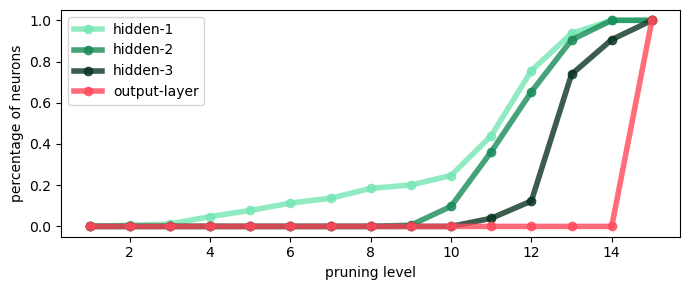
\includegraphics[width=0.9\linewidth]{input-view.png}
    \caption{    
    The figure depicts the separation of each level.
    The separation is calculated from the inputs of the network.
    On the x-axis, the pruning levels are displayed and on the y-axis the percentage of neurons that can be attributed to a task.
    }\label{fig:inview}
\end{figure}

In figure~\ref{fig:outview} the degree of separation is displayed for each layer from the view of the outputs.
The network in this case was taken from the experiment with three hidden layers.
The network separates at iteration 15.

In the first iteration, none of the layers were separated.
Already by the second iteration, around $30$\% of the neurons in the last hidden layer (hidden-3) belong to only one task.
This increase in the degree of separation of this layer looks logarithmic.
At iteration 7, where already $\sim80$\% of neurons in the last hidden layer belong to a task, the penultimate hidden layer (hidden-2) starts to separate.
With one iteration delay, the next hidden layer (hidden-1) starts to separate.
It tracks the layer \textit{hidden-2} in its rapid, s-curve-shaped growth.
Only at iteration 14, when over $90$\% of neurons are already attributable to a task, the input layer separates.
In this case, the separation describes the perspective from the outputs.
It does not take into account the knowledge, of which input neuron belongs to which task.

The same network but from the view of the inputs is displayed in figure~\ref{fig:inview}.
In this case, the separation is significantly slower in the beginning.
After iteration 10, the separation speeds up at iteration 15, the network is completely separated.
The difference in the degree of separation, depending on the point of view, could have several reasons.
It could be that the slower separation is due to the fact, that there are four inputs and only two outputs.
Therefore, for the neurons to be only connected to the inputs of one task, two instead of one weights have to be pruned.
Another possibility is that the weights in the first layer are higher in magnitude than the weights in the last layer.
This would result in stronger pruning in the last layer.
In the course of this thesis, these questions will not be further pursued.



\subsection{Performance of Lottery tickets}
One remaining question is if the networks still perform well when they split.
Are they better, equal, or worse in terms of the validation loss, compared to the other networks?

\begin{figure}[ht]
    \centering
    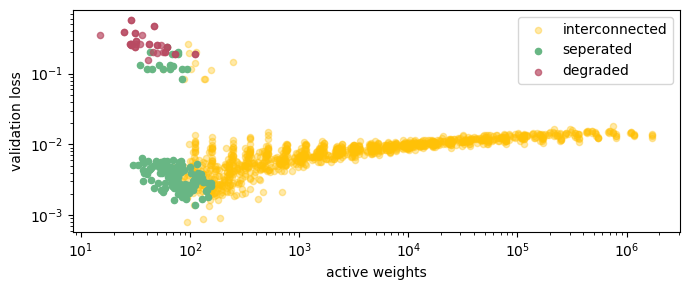
\includegraphics[width=0.9\linewidth]{performance.png}
    \caption{
        This figure visualizes the performance of the networks at each pruning level.
        On the x-axis, the number of active weight is displayed.
        On the y-axis, the validation loss is shown.
        Each dot represents a network at one stage.
        An experiment with 20 pruning levels is shown with 20 dots in this figure.
        The color refers to the state of the network at the iteration.
    }\label{fig:performance}
\end{figure}

To investigate the performance, the validation loss from the experiment with two hidden layers described in paragraph~\ref{two-hidden} was used.
In figure~\ref{fig:performance}, the validation loss is depicted on the y-axis.
On the x-axis, the number of active weights is displayed.
To get a better understanding of the performance of the networks, the loss was plotted at each iteration for each network.
Namely, for a network extended 20 times, there are 20 loss values, each plotted as a single point.
The color of the point represents if the network was interconnected (yellow), separated (green), or degraded (red) at the iteration the point refers to.
The loss value is calculated after the training and before the pruning of each iteration, as shown in the code snippet~\ref{code:imp}.

The bending line of yellow points demonstrates the consistent performance of the networks during the early iterations.
Likely due to early splitting, the networks remain at a validation loss of around $0.01$.
The loss decreases slightly over the pruning iterations.
A visible cluster of green dots sits at the end of the yellow line.
These dots represent the networks that are separated.
The iterations where the networks are separated are amongst the networks with the lowest loss.
This indicates that the separation of the networks is not merely a consequence of pruning to extremely high sparsities.
Rather, the separated networks still represent a well-performing function, even amongst the best-performing networks overall.

Interestingly, there is a second distinct cluster of networks.
It sits at the same number of active weights, however with significantly higher loss.
This cluster contains interconnected, separated, and degraded networks at seemingly even ratios.
Since the experiments were stopped as soon as a network degraded, the red points refer to losses immediately after the network degraded.
Even though the cluster looks compact along the y-axis it covers a fairly large range between 0.08 and 0.56 loss. These losses correspond to an accuracy of roughly $95$\% and $65$\% respectively.
The separated and interconnected networks still generally inhabit an area with lower loss than the degraded networks.


\section{Experiments on the MNIST-Fashion-MNIST Dataset}
Due to the success of the method in separating the neural network, the same was attempted on the more realistic dataset described in paragraph~\ref{sec:mnist}.
The experiments cannot be executed as systematically as before, due to significantly higher computational cost.
However, with experience gained from previous experiments, it was indeed possible to find separated networks.

The hyperparameters are mostly the same as in the previous experiments.
The network is trained with the ADAM optimizer and a learning rate of $0.001$.
Additionally, a larger batch size of 512 is selected, since the data is more diverse and there are significantly more samples.


The dataset includes 1568 input features and 20 output features

A network with shape $(1568, 784, 392, 20)$ was used for these experiments.
The architecture was selected to resemble the LeNet architecture used in \autocite{LTH} on the MNIST dataset.
The LeNet architecture has a shape of $(784, 300, 100, 10)$.
In preliminary experiments, the networks separated at significantly larger numbers of parameters.
Therefore, the pruning target was set to 600.
For the training, 20 pruning levels were selected, which resulted in a pruning rate of $p=0.3247$, similar to the experiments on the Moons-Circles dataset.
Further, for the first experiments, the data was normalized like the Moons-Circles dataset, namely to zero mean and unit variance.

With the described setup, the network was trained with three different seeds for the weight initialization.
\begin{figure}[ht]
    \centering
    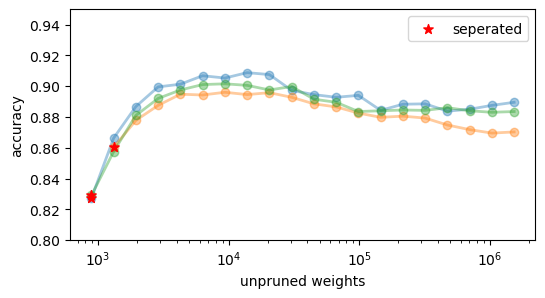
\includegraphics[width=.7\linewidth]{mnist-acc-largest-784-392.png}
    \caption{
        This figure shows the accuracy of three runs with the same hyperparameters but different seeds on the MNIST-Fashion-MNIST dataset.
        On the x-axis, the number of active weights is displayed.
        On the y-axis, the accuracy is shown.
        The dataset was normalized to zero mean and unit variance.
        Each line represents one run.
        The star indicates where the networks separated.
    }\label{fig:mnist-acc}
\end{figure}

In figure~\ref{fig:mnist-acc}, the accuracy of the three runs with different seeds is shown.
The red star shows where the networks separate.
The iteration where the networks separate is also always the last because after separation occurs, the training is stopped to save time.
When the networks split, the accuracy already is significantly lower than at the peak.
The best accuracy of a separated network amongst the shown runs is $\sim86$ percent.

\begin{figure}[ht]
    \centering
    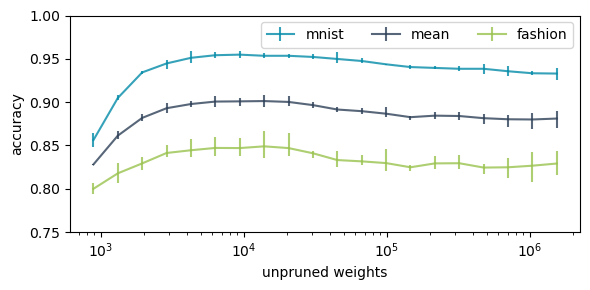
\includegraphics[width=.7\linewidth]{taskwise-acc.png}
    \caption{
        This figure shows the accuracy of the two tasks.
        Each line is an average of the three runs with different seeds.
        The error bars indicate minimum and maximum values.
        On the x-axis, the number of active weights is displayed.
        On the y-axis, the accuracy is shown.
    }\label{fig:taskwise-acc}
\end{figure}

The accuracy shown in figure~\ref{fig:mnist-acc} represents the average accuracy of both tasks.
The data in figure~\ref{fig:taskwise-acc} shows the accuracy of the tasks separately.
Since the tasks are not the same, it is to be expected that they do not exhibit the same performance.
The accuracy achieved on the MNIST task is more than $10$ percent higher than on the Fashion MNIST task.
Interestingly, when the number of parameters gets lower, the performance on the MNIST task worsens significantly faster than for the Fashion MNIST task.

The performance of the network is not satisfactory anymore at the time it separates.
However, the experiments shown here are only preliminary.
The networks indeed separate consistently, and they do far beyond trivial accuracies.
This gives reason to believe, that the separation can be achieved at competitive accuracy with improved hyperparameters or slight adaptations to the training.
This, however, is not pursued in the scope of this thesis.
The separation by itself, at non-trivial accuracy is considered a useful insight into the structure of the network.

\subsection{What does the model }


\subsection{Conclusion: Network Extension}
They always split

multiple this have to be given

enough overparameterization
pruning rate low enough
enough pruning levels

Not clear how the splitting happens
Maybe unzipping?
What about the reguriating tickets interpretation?
What about regularization, weight decay and so on?
